\section[The Riemann-Stieltjes Integral]{\hyperlink{toc}{The Riemann-Stieltjes Integral}}

\subsection{Definition of the Integral}
\begin{definition}{Partition}{6.1}
    A \textbf{partition} of $[a, b] \subset \RR$ is a set $\set{x_0, x_1, \ldots, x_n}$ (for some $n \in \NN$) such that:
    \begin{align*}
        a = x_0 \leq x_1 \leq x_2 \leq \ldots \leq x_{n-1} \leq x_n = b
    \end{align*}
    We can then write:
    \begin{align*}
        \Delta x_i = x_i - x_{i-1} 
    \end{align*}
\end{definition}

\begin{figure}[htbp]
    \centering
    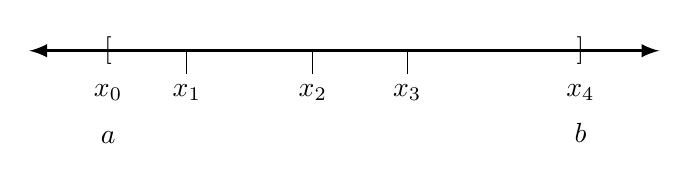
\begin{tikzpicture}[scale=2]
        \draw[very thick, latex-latex] (-2, 0) -- (2, 0);
        \node[] at (-1.5, 0) {$[$};
        \node[below] at (-1.5, -0.15) {$x_0$};
        \node[below] at (-1.5, -0.45) {$a$};
        \node[] at (1.5, 0) {$]$};
        \node[below] at (1.5, -0.15) {$x_4$};
        \node[below] at (1.5, -0.4) {$b$};
        \draw[] (-1, 0) -- (-1, -0.15);
        \node[below] at (-1, -0.15) {$x_1$};
        \draw[] (-0.2, 0) -- (-0.2, -0.15);
        \node[below] at (-0.2, -0.15) {$x_2$};
        \draw[] (0.4, 0) -- (0.4, -0.15);
        \node[below] at (0.4, -0.15) {$x_3$};
    \end{tikzpicture}
    \caption{Visualization of a partition $\set{x_0, x_1, x_2, x_3, x_4}$ of $[a, b]$. Note that the points in the partitions need not be equally spaced.}
    \label{fig27}
\end{figure}

\setcounter{rudin}{0}
\begin{definition}{Upper and Lower Sums}{6.1}
    Given $f: [a, b] \mapsto \RR$ and a partition $P$ of $[a, b]$ let:
    \begin{align*}
        M_i &= \sup\set{f(x): x_{i-1} \leq x \leq x_i}
        \\ m_i &= \inf\set{f(x): x_{i-1} \leq x \leq x_i}
    \end{align*}
    Then, we can define the \textbf{upper} and \textbf{lower sums}:
    \begin{align*}
        U(P, f) &= \sum_{i=1}^n M_i \Delta x_i
        \\ L(P, f) &= \sum_{i=1}^n m_i \Delta x_i
    \end{align*}
\end{definition}

\begin{figure}[htbp]
    \centering
    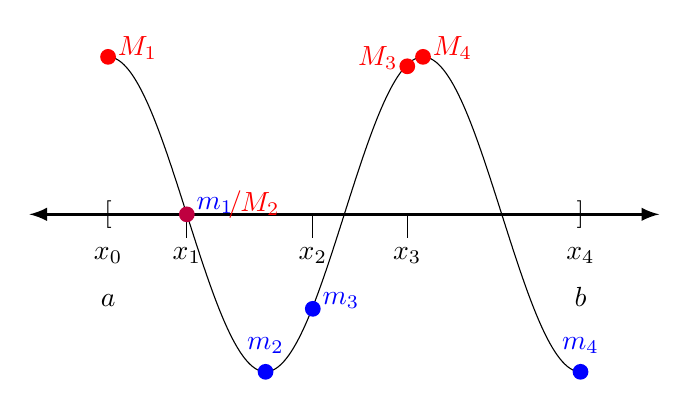
\begin{tikzpicture}[scale=2]
        \draw[very thick, latex-latex] (-2, 0) -- (2, 0);
        \node[] at (-1.5, 0) {$[$};
        \node[below] at (-1.5, -0.15) {$x_0$};
        \node[below] at (-1.5, -0.45) {$a$};
        \node[] at (1.5, 0) {$]$};
        \node[below] at (1.5, -0.15) {$x_4$};
        \node[below] at (1.5, -0.4) {$b$};
        \draw[] (-1, 0) -- (-1, -0.15);
        \node[below] at (-1, -0.15) {$x_1$};
        \draw[] (-0.2, 0) -- (-0.2, -0.15);
        \node[below] at (-0.2, -0.15) {$x_2$};
        \draw[] (0.4, 0) -- (0.4, -0.15);
        \node[below] at (0.4, -0.15) {$x_3$};
        \draw[] (-1, 0) sin (-1.5, 1);
        \draw[] (-1, 0) sin (-0.5, -1);
        \draw[] (0, 0) sin (-0.5, -1);
        \draw[] (0, 0) sin (0.5, 1);
        \draw[] (1, 0) sin (0.5, 1);
        \draw[] (1, 0) sin (1.5, -1);
        \node[circle, fill = red, minimum size = 0.2cm, inner sep = 0pt, label={[right, text=red]:$M_1$}] at (-1.5, 1) {};
        \node[circle, fill = purple, minimum size = 0.2cm, inner sep = 0pt, label={[right, text=blue]:$m_1$}] at (-1, 0) {};
        \node[right, text = red] at (-0.8, 0.06) {$/M_2$};
        \node[circle, fill = blue, minimum size = 0.2cm, inner sep = 0pt, label={[above, text=blue]:$m_2$}] at (-0.5, -1) {};
        \node[circle, fill = blue, minimum size = 0.2cm, inner sep = 0pt, label={[right, text=blue]:$m_3$}] at (-0.2, -0.6) {};
        \node[circle, fill = red, minimum size = 0.2cm, inner sep = 0pt, label={[left, text=red]:$M_3$}] at (0.4, 0.94) {};
        \node[circle, fill = red, minimum size = 0.2cm, inner sep = 0pt, label={[right, text=red]:$M_4$}] at (0.5, 1) {};
        \node[circle, fill = blue, minimum size = 0.2cm, inner sep = 0pt, label={[above, text=blue]:$m_4$}] at (1.5, -1) {};
        \end{tikzpicture}
    \caption{Example of a function $f$, a partition $P$ of $[a, b]$, and the $M_i, m_i$s for this choice of partition.}
    \label{fig28}
\end{figure}

\noindent By construction, it should be evident that $L(P, f) \leq U(P, f)$ for all $P, f$.

A natural question that arises from the form of the above expression is whether these are Riemann sums or not. Recall from first year calculus that we would choose the left endpoint, right endpoint, or some other arbitrary choice of a point in the subinterval. Here, we in a sense use a ``special case'' of the supremum/infimum. We will see that this choice is musch easier to use in proofs due to monotonicity properties. Namely, if we have a partition and add another point, then $U(P, f)$ can only decrease, and $L(P, f)$ can only increase (we will see this in a theorem soon)!


\setcounter{rudin}{0}
\begin{definition}{Upper/Lower Integrals and Riemann Integrability}{6.1}
    We define the \textbf{upper Riemann integral} to be:
    \begin{align*}
        \uint{a}{b} = \inf_P U(P, f).
    \end{align*}
    and the \textbf{lower Riemann integral} to be:
    \begin{align*}
        \lint{a}{b} = \sup_P L(P, f).
    \end{align*}
    Here, the infimum/supremum is taken over all partitions $P$. We say that $f$ is \textbf{Riemann integrable} on $[a, b]$, and write $f \in \R[a, b]$ if:
    \begin{align*}
        \uint{a}{b} = \lint{a}{b}
    \end{align*}
    which we can write as:
    \begin{align*}
        \int_{a}^{b} f dx \text{ or } \int_{a}^{b} f(x) dx
    \end{align*}
\end{definition}
\noindent Note that the choice of variable in the above definition is totally arbitrary. 

Also, note that while $f$ is not required to be continuous in the above definition, it is required to be bounded; else, $M_i$ and $m_i$ may not exist. Since $f$ is bounded, $U(P, f)$, $L(P, f)$ are bounded for all $P, f$ and hence we have a set of real numbers for which we may consider the supremum/infimium of by the LUB/GLB property of the reals. Since the upper/lower sums lie in a bounded interval, there is no questions about whether the lower/upper integrals exist. The question becomes whether they are equal or not. Before getting into further discussion on this topic, we discuss a bound:

\setcounter{rudin}{0}
\begin{theorem}{ML Bounds}{6.1}
    Let $m = \inf\set{f(x): a \leq x \leq b}$ and $M = \sup\set{f(x): a \leq x \leq b}$ (which exist by the boundedness of $f$). Then,
    \begin{align*}
        m(b - a) \leq L(P, f) \leq U(P, f) \leq M(b - a)
    \end{align*}
    For any choice of partition $P$.
\end{theorem}
\begin{nproof}
    For any $i$, we have that:
    \begin{align*}
        m \leq m_i \leq M_i \leq M
    \end{align*}
    Therefore:
    \begin{align*}
        \sum_{i=1}^n m \Delta x_i \leq \sum_{i=1}^n m_i \Delta x_i \leq \sum_{i=1}^n M_i \Delta x_i \leq \sum_{i=1}^n M \Delta x_i
    \end{align*}
    So we conclude that:
    \begin{align*}
        m(b - a) \leq L(P, f) \leq U(P, f) \leq M(b - a)
    \end{align*} \qed
\end{nproof}

\noindent Now that we have established the Riemann integral, a natural question is how can we extend this notion. In order to do so, we will use a montonically increasing function $\alpha: [a, b] \mapsto \RR$ (that is, $\alpha(x) \leq \alpha(y)$ for all $x \leq y$). Note that $\alpha$ need not be continuous. Indeed, compared to the Riemann integral where $\alpha(x) = x$ and was continuous, in this general setting, $\alpha$ is allowed to have jumps. This allows for certain benefits, as we will soon discuss. However, we note that $\alpha$ can only have a finite number of jumps.

\begin{ntheorem}{ 4.30}{}
    Let $\alpha: [a, b] \mapsto \RR$ be monotonic. Then, it can only have finitely many discontinities.
\end{ntheorem}
\begin{nproof}
    Assign a rational number $r(x)$ to each of the discontinuities of $\alpha$. Then, we have that:
    \begin{align*}
        \lim_{x \rightarrow r(x)^-} \alpha(x) < \alpha(x) < \lim_{x \rightarrow r(x)^+} \alpha(x)
    \end{align*}
    Since $x_1 < x_2$ implies $\lim_{x \rightarrow r(x_1)^+} \alpha(x) \leq lim_{x \rightarrow r(x_2)^-} \alpha(x)$, we have that $r(x_1) \neq r(x_2)$ if $x_1 \neq x_2$. We therefore have established a function $r$ from the set of discontinuities of $\alpha$ to the rationals. As the rationals are countable, the set of discontiuities of $\alpha$ are also countable. \qed
\end{nproof}

\noindent With this established, we now define the generalized Riemann-Stieltjes integral.

\begin{definition}{Riemann-Stieltjes Integral}{6.2}
    Let $\alpha: [a, b] \mapsto \RR$ be increasing, and given a partition $P$ of $[a, b]$, define:
    \begin{align*}
        \Delta \alpha_i = \alpha(x_i) - \alpha(x_{i-1}) (\geq 0)
    \end{align*}
    For bounded $f: [a, b] \mapsto \RR$, Let:
    \begin{align*}
        U(P, f, \alpha) &= \sum_{i=1}^n M_i \Delta \alpha_i
        \\ L(P, f, \alpha) &= \sum_{i=1}^n m_i \Delta \alpha_i
    \end{align*}
    We then take the infimum/supremum over partitions $P$ to get:
    \begin{align*}
        \uint{a}{b} f d\alpha &= \inf_P U(P, f, \alpha)
        \\ \lint{a}{b} &= \sup_P L(P, f, \alpha)
    \end{align*}
    If equal, we write their value as:
    \begin{align*}
        \int_a^b f d\alpha \text{ or } \int_a^b f(x)d\alpha(x)
    \end{align*}
    and we write that $f \in \R_\alpha[a, b]$. In the case where $\alpha(x) = x$, we recover the Riemann integral.
\end{definition}

\noindent Why is this definition useful? What does it accomplish for us that the original Riemann integral does not? We consider a physically motivating example. Suppose we have a thin wire with varying mass density $\rho(x)$. If we wanted to calculate the mass density of the wire, we would integrat the density $\rho(x)$ over the length of the wire. Now, suppose our wire consists of steel of continuously varying mass density, as well as beads/point masses placed on certain locations of the wire. The Riemann integral cannot handle these point masses, but the Riemann-Stieltjes integral can deal with this case if we use an $\alpha$ with discontinuities in it. Hence, the Riemann-Stieltjes integral allows us to handle cases where we both have continuous and discrete masses to integrate over. It acts as a bridge between Riemann and Lebesgue integration (the latter of which will be the subject of a later course in measure theory).

We now will answer the question: ``for what choices of $f, \alpha$ is $f$ Riemann-Stieltjes integrable?''

\subsection{Criterion for Integrability}

\begin{definition}{Refinements and Common Refinemnet}{6.3}
    $P^*$ is a \textbf{refinement} of $P$ if $P \subset P^*$ and $P, P^*$ are partitions. The common refinemnet of $P_1, P_2$ is $P^* = P_1 \cup P_2$.
\end{definition}

\begin{theorem}{}{6.4}
    If $P^*$ is a refinemne tof $P$, then:
    \begin{align*}
        L(P, f, \alpha) \leq L(P^*, f, \alpha) \leq U(P^*, f, \alpha) \leq U(P, f, \alpha)
    \end{align*}
\end{theorem}

\noindent As a remark, when we take infimums/supremums over partitions $P$ to obtain the upper/lower Riemann-Stieltjes integals, we are taking refinements.

Also, note that the above theorem does \textit{not} apply to (right-hand, left-hand, midpoint, arbitrary) Riemann sums, and is a consequence of the choice of upper/lower sums with supremums/infimums taken over the subintervals.

\begin{nproof}
    It suffices to consider $P^*$ with a single extra point $x_{i - 1} < x^* < x_i$, and then the genral case follows by induction.

    For the case where $\alpha(x) = x$, the refinement adds $(m^* - m_i)(x^* - x_{i-1}) \geq 0$. 

    For the general case, we have that:
    \begin{align*}
        L(P^*, f, \alpha) - L(P, f, \alpha) &= \left(m^*(\alpha(x^*) - \alpha(x_{i-1})) + m_i(x^* - x_{i-1}) \right)- m_i(\alpha_{x_i} - \alpha_{x_{i-1}})
        \\ &= \left(m^*(\alpha(x^*) - \alpha(x_{i-1})) + m_i(x^* - x_{i-1}) \right)
        \\ &- m_i\left[(\alpha(x^*) - \alpha(x_{i-1})) + (\alpha(x_i) - \alpha(x^*))\right]
        \\ &= (m^* - m_i)(\alpha(x^*) - \alpha(x_i))
    \end{align*}
    $\alpha$ is montonically increasing, so $x^* \geq x_i$ implies that the second term is positive. Furthermore, $m^* \geq m_i$ as $\inf\set{f(x): x \in [x_{i-1}, x^*]} \geq \inf\set{f(x): x \in [x_{i-1}, x_i]}$. It follows that:
    \begin{align*}
        L(P^*, f, \alpha) - L(P, f, \alpha) \geq 0
    \end{align*} 
    and the proof for $U(P^*, f, \alpha) - U(P, f, \alpha) \leq 0$ follows analogously. \qed
\end{nproof}
\begin{figure}[htbp]
    \centering
    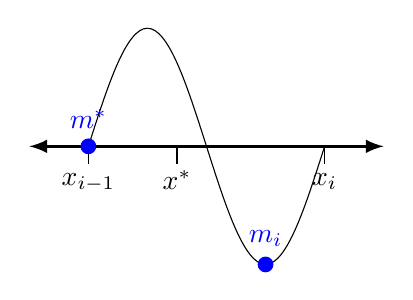
\begin{tikzpicture}[scale=1.5]
        \draw[latex-latex, very thick] (-1.5, 0) -- (1.5, 0);
        \draw[] (-1, 0) sin (-0.5, 1);
        \draw[] (0, 0) sin (-0.5, 1);
        \draw[] (0, 0) sin (0.5, -1);
        \draw[] (1, 0) sin (0.5, -1);
        \draw[] (-1, 0) -- (-1, -0.15);
        \draw[] (1, 0) -- (1, -0.15);
        \node[below] at (-1, -0.15) {$x_{i-1}$};
        \node[below] at (1, -0.15) {$x_i$};
        \draw[] (-0.25, 0) -- (-0.25, -0.15);
        \node[below] at (-0.25, -0.12) {$x^*$};
        %\node[circle, fill = red, minimum size = 0.2cm, inner sep = 0pt, label={[right, text=red]:$M_{i\text{original}}/M_{i\text{new}}$}] at (-0.5, 1) {};
        \node[circle, fill = blue, minimum size = 0.2cm, inner sep = 0pt, label={[above, text=blue]:$m_{i}$}] at (0.5, -1) {};
        %\node[circle, fill = red, minimum size = 0.2cm, inner sep = 0pt, label={[right, text=red]:$M_{i+1\text{new}}$}] at (-0.25, 0.7) {};
        \node[circle, fill = blue, minimum size = 0.2cm, inner sep = 0pt, label={[above, text=blue]:$m^*$}] at (-1, 0) {};
    \end{tikzpicture}
    
    \caption{Visualization of the effect of adding an extra point $x^*$ to the partition $P$. We can see that this has the net effect of increasing $L(P, f, \alpha)$ as $m^* \geq m_i$.}
    \label{fig29}
\end{figure}

\newpage 
Note that as a point of notation, if $f, \alpha$ are fixed, we sometimes can write $L(P), U(P)$ in place of $L(P, f, \alpha)$ and $U(P, f, \alpha)$. Sometimes where the context is clear, it is also common to write $\R(\alpha)$ in place of $\R_\alpha[a, b]$. 

\begin{theorem}{}{6.5}
    $\lint{a}{b} f d\alpha \leq \uint{a}{b} f d\alpha$.
\end{theorem}
\begin{nproof}
    For partitions $P_1, P_2$, let $P^* = P_1 \cup P_2$ be the common refinement. By Theorem \ref{thm:6.4}, we have that:
    \begin{align*}
        L(P_1) \leq L(P^*) \leq U(P^*) \leq U(P_2)
    \end{align*}
    And in particular, $L(P_1) \leq U(P_2)$. Therefore, for any fixed $P_2$, $U(P_2)$ is an upper bound on the set of all lower sums. As the supremum is the least upper bound, we have that:
    \begin{align*}
        \sup_{P_1} L(P_1) \leq U(P_2)
    \end{align*}
    Therefore, as $\sup_{P_1} L(P_1)$ is a lower bound on the set of all upper sums, and the infimum is the greatest lower bound, we have that:
    \begin{align*}
        \sup_{P_1} L(P_1) \leq \inf_{P_2} U(P_2)
    \end{align*}
    So therefore:
    \begin{align*}
        \lint{a}{b} f d\alpha \leq \uint{a}{b} f d\alpha
    \end{align*}
    as claimed. \qed
\end{nproof}

\begin{theorem}{\texorpdfstring{$\e$}{e}-Criterion for Integrability}{6.6}
    $f \in \R_\alpha[a, b]$ if and only if for all $\e > 0$, there exists a partition $P_\e$ of $[a, b]$ such that $U(P_\e) - L(P_\e) < \e$. 
\end{theorem}
\begin{nproof}
    $\boxed{\implies}$ By hypothesis, $\sup_P L(P) = \int_a^b fd\alpha = \inf_P U(P)$. Let $\e > 0$. Then by the property of sup/inf, there exist $P_1, P_2$ such that:
    \begin{align*}
        \int_a^b f d\alpha - L(P_1) &< \frac{\e}{2}
        \\ U(P_2) - \int_a^b f d\alpha &< \frac{\e}{2}
    \end{align*}
    Adding the first inequality to the second, we get:
    \begin{align*}
        U(P_2) - L(P_1) < \e
    \end{align*}
    Letting $P^* = P_1\cup P_2$, by Theorem \ref{thm:6.4} we have that:
    \begin{align*}
        U(P^*) - L(P^*) \leq U(P_2) - L(P_1) < \e
    \end{align*}
    which proves the claim.

    $\boxed{\impliedby}$ Let $\e > 0$ Then by Theorem \ref{thm:6.5} we have that:
    \begin{align*}
        0 \leq \uint{a}{b} f d\alpha - \lint{a}{b} f d\alpha
    \end{align*}
    and furthermore:
    \begin{align*}
        0 \leq \uint{a}{b} f d\alpha - \lint{a}{b} f d\alpha \leq U(P_\e) - L(P_\e) < \e
    \end{align*}
    Where the second inequality is true for any choice of partition. $\e$ is arbitrary, so we conclude that:
    \begin{align*}
        \uint{a}{b} f d\alpha - \lint{a}{b} f d\alpha = 0
    \end{align*}
    And therefore $\uint{a}{b} f d\alpha = \lint{a}{b} f d\alpha$, and $f \in \R_\alpha[a, b]$. \qed
\end{nproof}

\noindent Theorem 6.7 is a little technical, so we shall skip it for now.

\stepcounter{rudin}
\begin{theorem}{Continuity implies integrability}{6.8}
    If $f$ is continuous on $[a, b]$, then $f \in \R_\alpha[a, b]$. 
\end{theorem}
\noindent Note in the above theorem that we make no assumptions on $\alpha$, only that (of course) it is monotonic.
\begin{nproof}
    By definition, $U(P) - L(P) = \sum_{i=1}^n (M_i - m_i)\Delta \alpha_i$. The idea will be to choose small intervals to make these differences small. Since $[a, b]$ is compact, $f$ is uniformly continuous by Theorem \ref{thm:4.19}. So, for all $\eta > 0$, there exists $\delta > 0$ such that $\abs{f(x) - f(t)} < \eta$ if $\abs{x - t} < \delta$. Thus, if $P$ is constructed such that $\Delta x_i < \delta$ then $M_i - m_i < \eta$. We then have that:
    \begin{align*}
        U(P) - L(P) \leq \sum_{i=1}^n \eta \Delta \alpha_i = \eta \sum_{i=1}^n (\alpha(x_{i}) - \alpha(x_{i-1})) = \eta\left(\alpha(b) - \alpha(a)\right)
    \end{align*}
    Where in the last equality we use the fact that we have a telescoping sum. Given $\e > 0$, we choose $\eta < \frac{\e}{\alpha(b) - \alpha(a)}$. With this choice of partition with $\Delta x_i < \delta = \delta(\eta)$, we have that:
    \begin{align*}
        U(P) - L(P) < \e
    \end{align*}
    and we conclude that $f \in \R_\alpha[a, b]$ by Theorem \ref{thm:6.6}. \qed
\end{nproof}
\noindent A natural question is ``what $f$s are Riemann integrable in general?'' The answer turns out to be ``if $f$ is continuous almost everywhere''. This sounds handwavy, but has a precise definition; although it is not covered in this course, one can refer to Rudin 11.33(b) for details. 

\begin{theorem}{}{6.9}
    If $f$ is monotone on $[a, b]$ and $\alpha$ is continuous on $[a, b]$m then $f \in \R_\alpha[a, b]$. 
\end{theorem}
\noindent In the proof of Theorem \ref{thm:6.8}, we used the continuity of $f$ to bound the maximum/minimum on each subinterval. Here, $f$ is no longer continuous, so we cannot control the maximum/minimum. Instead, we will use the continuity of $\alpha$ to control the size of the $\Delta \alpha$s. 
\begin{nproof}
    Given $n \in \NN$, choose $P$ such that $\Delta \alpha_i = \frac{\alpha(b) - \alpha(a)}{n}$ for all $i \in {1, \ldots, n}$. Note that such a choice is possible by the continuity of $\alpha$ and the IVT (Theorem \ref{thm:4.23}). We then have that:
    \begin{align*}
        U(P) - L(P) = \sum_{i=1}^n (M_i - m_i)\Delta \alpha_i = \frac{\alpha(b) - \alpha(a)}{n}\sum_{i=1}^n (M_i - m_i)
    \end{align*}
    Suppose (WLOG) that $f$ is an increasing function. Then, $M_i = f(x_i)$ and $m_i = f(x_{i-1})$ due to the monotone increasing property. Hence:
    \begin{align*}
        U(P) - L(P) = \frac{\alpha(b) - \alpha(a)}{n}\sum_{i=1}^n f(x_i) - f(x_{i-1}) = \frac{\alpha(b) - \alpha(a)}{n}\left[f(b) - f(a)\right]
    \end{align*}
    Where in the last equality we use the fact that the sum telescopes. If $\alpha(b) = \alpha(a)$, then $U(P) - L(P) = 0$ and the claim immediately follows. If $\alpha(b) > \alpha(a)$, then the claim follows by choosing $n > \frac{1}{\e}\frac{f(b) - f(a)}{\alpha(b) - \alpha(a)}$ (that is, selecting a partition $P$ with sufficiently large $n$), from which it follows that:
    \begin{align*}
        U(P) - L(P) < \e
    \end{align*}
    and hence $f \in \R_\alpha[a, b]$ by Theorem \ref{thm:6.6}. \qed
\end{nproof}
\begin{figure}[htbp]
    \centering
    \begin{tikzpicture}[scale=2]
        \draw[-latex, very thick] (0, 0) -- (2, 0);
        \draw[-latex, very thick] (0, 0) -- (0, 2);
        \foreach \i in {0.5,0.7,...,1.7}{ 
            \draw[] (0, \i) -- (-0.15, \i);
        }
        \filldraw[] (0.5, 0.5) circle (1pt);
        \filldraw[] (1.7, 1.7) circle (1pt);
        \draw[] (0.5, 0) -- (0.5, -0.15);
        \draw[] (1.7, 0) -- (1.7, -0.15);
        \node[below] at (0.5, -0.16) {$a$};
        \node[below] at (1.7, -0.13) {$b$};
        \node[left] at (-0.15, 0.5) {$\alpha(a)$};
        \node[left] at (-0.15, 1.7) {$\alpha(b)$};
        \draw[dashed] (0, 0.5) -- (0.5, 0.5);
        \draw[dashed] (0.5, 0) -- (0.5, 0.5);
        \draw[dashed] (0, 0.7) -- (0.86, 0.7);
        \draw[dashed] (0.86, 0) -- (0.86, 0.7);
        \draw[dashed] (0, 0.9) -- (0.95, 0.9);
        \draw[dashed] (0.95, 0) -- (0.95, 0.9);
        \draw[dashed] (0, 1.1) -- (1.15, 1.1);
        \draw[dashed] (1.15, 0) -- (1.15, 1.1);
        \draw[dashed] (0, 1.3) -- (1.3, 1.3);
        \draw[dashed] (1.3, 0) -- (1.3, 1.3);
        \draw[dashed] (0, 1.5) -- (1.36, 1.5);
        \draw[dashed] (1.36, 0) -- (1.36, 1.5);
        \draw[dashed] (0, 1.7) -- (1.7, 1.7);
        \draw[dashed] (1.7, 0) -- (1.7, 1.7);
        \draw [] (0.5 , 0.5) to [ curve through ={(0.8, 0.6)..(1, 1)..(1.25, 1.2)..(1.4, 1.6)}] (1.7, 1.7);
    \end{tikzpicture}
    
    \caption{Visualization of the idea of the proof of Theorem \ref{thm:6.9}. We chop up $[\alpha(a), \alpha(b)]$ into equal sized subintervals.}
    \label{fig30}
\end{figure}

\begin{theorem}{}{6.10}
    Suppose $f: [a, b] \mapsto \RR$ is bounded and has finitely many discontinuities. Suppose $\alpha$ is continuous at every point where $f$ is not. Then, $f \in \R_\alpha[a, b]$. 
\end{theorem}

\begin{nproof}
    As has become standard, we will be applying Theorem \ref{thm:6.6}. We have that:
    \begin{align*}
        U(P) - L(P) = \sum_{i=1}^n (M_i - m_i)\Delta \alpha_i
    \end{align*}
    Let $\e > 0$, and let $E = \set{e_1, \ldots e_k}$ be the set of points where $f$ is not continuous. $\alpha$ is continuous at each $e_j$ by hypothesis. Therefore, there exists disjoint intervals $(u_j, v_j)$ that cover points in $E$, such that $u_j < e_j < v_j$ and $\alpha(v_j) - \alpha(v_j) < \e$ (by the continuity of $\alpha$). Let $K = [a, b] \cap \left(\bigcup_{j=1}^k (u_j, v_j)\right)^c$. $K$ is a compact set as it is a finite union of closed intervals. $f$ is continuous on $K$ by hypothesis, so $f$ is uniformly conitnuous on $K$ by Theorem \ref{thm:4.19}. Hence, there exists $\delta > 0$ such that for $s, t \in K$, $\abs{s - t} < \delta \implies \abs{f(s) - f(t)} < \e$. We then form a partition $P = \set{x_1, \ldots, x_n}$ to consist of $\set{u_1, v_1, \ldots, u_k, v_k}$ and additional points in $K$ with $\delta x_i < \delta$. For such $i$, $f$ is continuous on the subinterval and hence $M_i - m_i < \e$. For the other intervals $[u_j, v_j]$, we have that $M_j - m_j \leq 2M$ where $M = \sup\set{\abs{f(x)}: x \in [a, b]}$ and that $\Delta \alpha_j < \e$. Therefore, we have that:
    \begin{align*}
        0 \leq U(P) - L(P) &= \sum_{i=1}^n (M_i - m_i)\Delta \alpha_i
        \\ &\leq 2M\e + \e\left(\alpha(b) - \alpha(a)\right)
    \end{align*}
    Where the first term comes from the $[u_j, v_j]$s and the second term is the maximum possible value from the subintervals of $K$. By choosing $\e$ small enough, the RHS is small as desired for some choice of $P$. Hence, $U(P) - L(P) < \e$ for some $P$ and hence $f \in \R_\alpha[a, b]$. \qed
\end{nproof}
A natural question that arises is ``what if $f$ and $\alpha$ are discontinuous at the same point?'' In this case, we can construct functions such that $f \notin \R_\alpha[a, b]$ (see HW1Q5).
\begin{figure}[htbp]
    \centering
    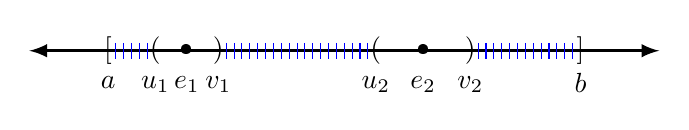
\begin{tikzpicture}[scale=2]
        \draw[latex-latex, very thick] (-2, 0) -- (2, 0);
        \node[] at (-1.5, 0) {$[$};
        \node[] at (1.5, 0) {$]$};
        \node[] at (-1.2, 0) {$($};
        \node[] at (-1, 0) {\textbullet};
        \node[] at (-0.8, 0) {$)$};
        \node[] at (0.2, 0) {$($};
        \node[] at (0.5, 0) {\textbullet};
        \node[] at (0.8, 0) {$)$};
        \foreach \i in {-1.45, -1.4, ..., -1.21} {
            \draw[blue] (\i, 0.05) -- (\i, -0.05);
        }
        \foreach \i in {-0.75, -.7, ..., 0.19} {
            \draw[blue] (\i, 0.05) -- (\i, -0.05);
        }
        \foreach \i in {0.85, 0.9, ..., 1.49} {
            \draw[blue] (\i, 0.05) -- (\i, -0.05);
        }
        \node[below] at (-1.5, -0.1) {$a$};
        \node[below] at (-1.2, -0.1) {$u_1$};
        \node[below] at (-1, -0.1) {$e_1$};
        \node[below] at (-0.8, -0.1) {$v_1$};
        \node[below] at (0.2, -0.1) {$u_2$};
        \node[below] at (0.5, -0.1) {$e_2$};
        \node[below] at (0.8, -0.1) {$v_2$};
        \node[below] at (1.5, -0.08) {$b$};
    \end{tikzpicture}
    \caption{Visualization of how $[a, b]$ gets split up in the proof of Theorem \ref{thm:6.10}. $K$ consists of the union of the closed intervals marked in blue.}
    \label{fig31}
\end{figure}

\begin{theorem}{}{6.11}
    If $f \in \R_\alpha[a, b]$, $m \leq f(x) \leq M$ for all $x \in [a, b]$, and $\phi$ is continuous on $[m, M]$, then $\phi \circ f \in \R_\alpha[a, b]$. 
\end{theorem}
\begin{nproof}
    Not covered in lecture, see Rudin. \qed
\end{nproof}

\noindent As an example of the above theorem, suppose we have that $f \in \R(\alpha)$. Then, we have that $f^2 \in \R(\alpha)$ and $\abs{f} \in \R(\alpha)$ as $\phi(x) = x^2$ and $\phi(x) = \abs{x}$ are both continuous functions.

\subsection{Properties of the Integral}
\begin{theorem}{Linearity and Related Properties}{6.12}
\begin{enumerate}
    \item Suppose $f_1 \in \R_\alpha[a, b]$ and $f_2 \in \R_\alpha[a, b]$. Then, $f_1 + f_2 \in \R_\alpha[a, b]$ and $cf_1 \in \R_{[a,b]}(\alpha)$ for all $c \in \RR$. Furthermore:
    \begin{align*}
        \int_a^b(f_1 + f_2) d\alpha = \int_a^b f_1 d\alpha + \int_a^b f_2d\alpha \text{ and } \int_a^b cf_1 d\alpha = c\int_a^b f_1d\alpha
    \end{align*}
    \item Suppose $f_1, f_2 \in \R_\alpha[a, b]$ and $f_1(x) \leq f_2(x)$ for all $x \in [a, b]$. Then,
    \begin{align*}
        \int_a^b f_1 d\alpha \leq \int_a^b f_2d\alpha
    \end{align*}
    \item If $f \in \R_\alpha[a, b]$ and $c \in (a, b)$, then $f \in \R_\alpha[a, c] \cap \R_\alpha[c, b]$ and furthermore:
    \begin{align*}
        \int_a^b f d\alpha = \int_a^c f d\alpha + \int_c^b f d\alpha
    \end{align*}
    \item If $f \in \R_\alpha[a, b]$ and $\abs{f(x)} \leq M$ for all $x \in [a, b]$, then:
    \begin{align*}
        \abs{\int_a^b f d\alpha} \leq M(\alpha(b) - \alpha(a))
    \end{align*}
    \item If $f \in \R_{\alpha_1}[a, b]$ and $f \in \R_{\alpha_2}[a, b]$, then $f \in \R_{\alpha_1 + \alpha_2}[a, b]$ and $f \in \R_{c\alpha_1}[a, b]$ for all $c \geq 0$. Furthermore:
    \begin{align*}
        \int_a^b f d\alpha_1 + \int_a^b f d\alpha_2 = \int_a^b f d(\alpha_1 + \alpha_2) \text{ and } \int_a^b f d(c\alpha_1) = c\int_a^b f d\alpha_1
    \end{align*}

\end{enumerate}
\end{theorem}
\begin{nproof}
    \begin{enumerate}
        \item See Rudin and HW2Q1.
        \item We have that $L(P, f_1) \leq L(P, f_2)$ for all partitions $P$ as $\inf\set{f_1(x): x \in [x_{i-1}, x_i]} \leq \inf\set{f_2(x): x \in [x_{i-1}, x_i]}$ for all $i$ (as $f_1(x) \leq f_2(x)$). Therefore, we have that:
        \begin{align*}
            \int_a^b f_1 d\alpha = \sup_P L(P, f_1) \leq \sup_P L(P, f_2) = \int_a^b f d\alpha.
        \end{align*}
        \item Exercise (see HW2Q1 for the $\uint{a}{b}$ case)
        \item Consider any partition $P$ of $[a, b]$. Let $M = \sup\set{\abs{f(x): x \in [a, b]}}$. We then have that (using the ML bound from Theorem \ref{thm:6.1}):
        \begin{align*}
            -M[\alpha(b) - \alpha(a)] = \sum_{i=1}^n(-M)\Delta \alpha_i \leq \sum_{i=1}^n M_i \Delta \alpha_i = L(P, f, \alpha) \leq \int_a^b fd\alpha 
            \\ \leq U(P, f, \alpha) = \sum_{i=1}^n M_i \Delta \alpha_i \leq \sum_{i=1}^n M\Delta \alpha_i = M[\alpha(b) - \alpha(a)].
        \end{align*}
        \item We prove the first (additivity) statement. Let $\e > 0$. Choose $P_i, i \in \set{1, 2}$ (By Theorem \ref{thm:6.6}) such that \begin{align*}
            U(P_i, f, \alpha_i) - L(P_i, f, \alpha_i) < \frac{\e}{2} 
        \end{align*}   
        Let $P = P_1 \cup P_2$. Then, by Theorem \ref{thm:6.4}, we have that:
        \begin{align*}
            U(P^*, f, \alpha_i) - L(P^*, f, \alpha_i) < \frac{\e}{2}
        \end{align*}
        Adding the two expressions (for $i = 1, 2$) together, we have:
        \begin{align*}
            U(P^*, f, \alpha_1 + \alpha_2) - L(P^*, f, \alpha_1 + \alpha_2) < \e
        \end{align*}
        So $f \in \R_{\alpha_1 + \alpha_2}[a, b]$ by Theorem \ref{thm:6.6}. Furthermore, We have that:
        \begin{align*}
            \int_a^b f d(\alpha_1 + \alpha_2) \leq U(P^*, f, \alpha_1 + \alpha_2) = U(P^*, f, \alpha_1) + U(P^*, f, \alpha_2) < \int_a^b f d\alpha_1 + \int_a^b fd\alpha_2 + \e
        \end{align*}
        where we apply the inequality of $U(P^*, f, \alpha_i) < \int_a^b f d\alpha_i + \frac{\e}{2}$ in the last line. Similarly, we have that:
        \begin{align*}
            \int_a^b fd(\alpha_1 + \alpha_2) \geq L(P^*, f, \alpha_1 + \alpha_2) = L(P^*, f, \alpha_1) + L(P, f, \alpha_2) > \int_a^b fd\alpha_1 + \int_a^b fd\alpha_2 - \e
        \end{align*}
        Since $\e$ is arbitrary, we therefore conclude that:
        \begin{align*}
            \int_a^b f d(\alpha_1 + \alpha_2) = \int_a^b fd\alpha_1 + \int_a^b fd\alpha_2
        \end{align*} \qed
    \end{enumerate}
\end{nproof}

\begin{theorem}{}{6.13}
    \begin{enumerate}
        \item Suppose $f, g \in \R(\alpha)$. Then, $fg \in \R(\alpha)$.
        \item Suppose $f \in \R(\alpha)$. Then, $\abs{f} \in \R(\alpha)$ and $\abs{\int_a^b fd\alpha} \leq \int_a^b \abs{f}d\alpha$.
    \end{enumerate}
\end{theorem}
\begin{nproof}
    \begin{enumerate}
        \item By Theorem \ref{thm:6.12}(a), $f \pm g \in \R(\alpha)$, so by Theorem \ref{thm:6.11}, $(f \pm g)^2 \in \R(\alpha)$. Since $(f+g)^2 - (f-g)^2 = 4fg$, we then have that:
        \begin{align*}
            \frac{(f+g)^2 + (f-g)^2}{4} = fg \in \R(\alpha)
        \end{align*}
        \item By Theorem \ref{thm:6.11}, $\abs{f} \in \R(\alpha)$ letting $\phi(t) = \abs{t}$. Let $c = \sgn\left(\int_a^b f d\alpha\right) \in \set{-1, 0, 1}$. Then, we have that:
        \begin{align*}
            \abs{\int_a^b fd\alpha} = c\int_a^b d\alpha = \int_a^b cfd\alpha \leq \int_a^b \abs{f}d\alpha
        \end{align*}
        Where we use Theorem \ref{thm:6.12}(a) in the second equality, and Theorem \ref{thm:6.12}(b) in the last inequality (as $cf \leq \abs{f}$). \qed
    \end{enumerate}
\end{nproof}

\setcounter{rudin}{14}

\begin{theorem}{}{6.15}
    Suppose $f$ is bounded on $[a, b]$, $s \in (a, b)$, and $f$ is continuous at $s$. Let:
    \begin{align*}
        \alpha(x) = \begin{cases}
            0 & x \leq s
            \\ 1 & x > s
        \end{cases}
    \end{align*}
    Then, $\int_a^b fd\alpha = f(s)$ (and in particular, $f \in \R(\alpha)$).
\end{theorem}

\noindent This result is interesting, and some remarks on the nature of this theorem are in order. Firstly, by Theorem 4.29 (not covered in Lecture, see Rudin), since $\alpha$ is monotonically increasing, we have that $\lim_{t \rightarrow x^+}\alpha(t) = \alpha(x^+)$ and $\lim_{t \rightarrow x^-}\alpha(t) = \alpha(x^-)$ exist at every $x \in (a, b)$ and $\alpha(x^-) \leq \alpha(x) \leq \alpha(x^+)$. Secondly, Note that Rudin defines $\alpha$ in the above Theorem to be left contiuous, but in probability theory, it is conventional to use a right continuous (i.e. $\alpha(x) = \alpha(x^+)$ for all $x \in (a, b)$). We leave it as an exercise to prove the theorem for the case of a right continuous $\alpha$ (the strategy and result are identitcal).

Any physicists looking at the result of the Theorem will note that it looks very much like the ``Dirac Delta'' function; indeed, this choice of $\alpha$ is making rigorous the notion of a $\delta$ function where:
\begin{align*}
    \int_a^b f(x)\delta(x - s) = f(s)
\end{align*}
We leave it as a homework exercise (HW2Q2) to prove that no such function can actually exist. This step-function method is one way to make the $\delta$ function well-defined; other methods include taking the limit of a bell curve, or bringing in the theory of distributions (the latter which is most definitely outside the scope of this course).

Finally, we note that this example really shows off something that the Riemann integral cannot reproduce; the incorporation of ``discrete'' points.

\subsection{Integration and Differentiation}

